% !TEX root =  master.tex

\chapter{Grundlagen der Visualisierung}
% Einleitung
Das Ziel dieses Projektes liegt in der Erstellung eines hochwertigen Lehrvideos, um den komplexen Sachverhalt der Scheduling Algorithmen von Betriebssystemen intuitiv darzustellen, sodass interessierte Zuschauer relevante Sachverhalte schnell verstehen können. Um für den Lernenden ein Lehrvideo mit möglichst hoher Qualität anbieten zu können, ist eine Beschäftigung mit theoretischen Grundlagen der Visualisierung, den Animationen und anderen Aspekten der Audio und Farbgestaltung unabdingbar. Daher wird im folgenden auf grundlegende Theorien in einer Literaturrecherche eingegangen, welche direkt in das von uns produzierten Lehrvideo eingebracht werden. 

% Bestätigung für Animationsvideo mit kurzem Disclaimer
Unsere Herangehensweise ein Lehrvideo zu erstellen, wird durch die Dual-Coding-Theorie von Allan Paivio bestätigt, welche besagt, dass Informationen besser verarbeitet und erinnert werden können, wenn diese sowohl visuell als auch verbal aufbereitet werden \autocite{paivio_dual_1991}. Dies ist ein Kernaspekt von Lehrvideos und wird umgestzt, indem neben visuellen Darstellungen wie Diagrammen oder animierten Algorithmen diese stets zugleich auf der Tonspur erklärt werden. Laut der Cognitive Load Theorie von John Sweller ist hierbei allerdings darauf zu achten, dass die kognitive Belastung des Lernenden berücksichtigt wird. Um ein effektives Lehrvideo zu erstellen, ist es entscheidend, eine Ausgewogenheit zwischen informativen Inhalten und überladenen Darstellungen zu finden \autocite{sweller_cognitive_2011}. 
Animationen können hierbei helfen komplexe Konzepte in einfach zu verstehende visuelle Elemente zu zerlegen, wodurch die kognitive Belastung reduziert werden kann. Um den Lernenden hierbei jedoch nicht kognitiv zu überlasten, ist es essentiell, dass Animationen stets passend und synchron zu der Tonspur angeordnet sind und diese beiden Komponenten nicht voneinander abweichen. Sollte dies doch der Fall sein, kann Verwirrtheit oder eine kognitiver Leistungsüberschreitung des Lernenden entstehen, wodurch die vermittelten Inhalte nicht zielgerichtet aufgenommen werden können \autocite{sweller_cognitive_2011}. 

% Möglichkeit Überforderung zu vermeiden
Eine Möglichkeit diese kognitive Überlastung zu vermeiden, ist die Anwendung der Multimedia Prinzipien von Richard E. Mayer. Dieser erarbeitete, dass eine angemessene Kombination von Text, Bildern und Animationen das Lernen deutlich verbessern kann, da Lehrinhalte hierduch prägnanter dargestellt werden können \autocite{mayer_multimedia_2002}. Insbesondere das Kontiguitätsprinzip, welches besagt, dass verbundene Text- und Bildinformationen zeitlich und räumlich nahe präsentiert werden sollten, ist für die Gestaltung von Bildungsanimationen relevant. Durch einen dezent animierten Text können grafische Vorgänge parallel zur Tonspur beschrieben werden. Der Lernende kann sich diesen Text nun im eigenen Tempo durchlesen ohne bei einer kurzen Unaufmerksamkeit das Verständnis für den gesamten Sachverhalt zu verlieren. Da es sich hierbei um ein zentrales Prinzip handelt, wird dieses innerhalb unseres Lehrvideos ebenfalls zahlreich umgesetzt. 

% Screenshot einfügen mit Beschreibung. Etwas mit Grafik & animiertem Text dazu
\begin{figure}[h]
	\centering
	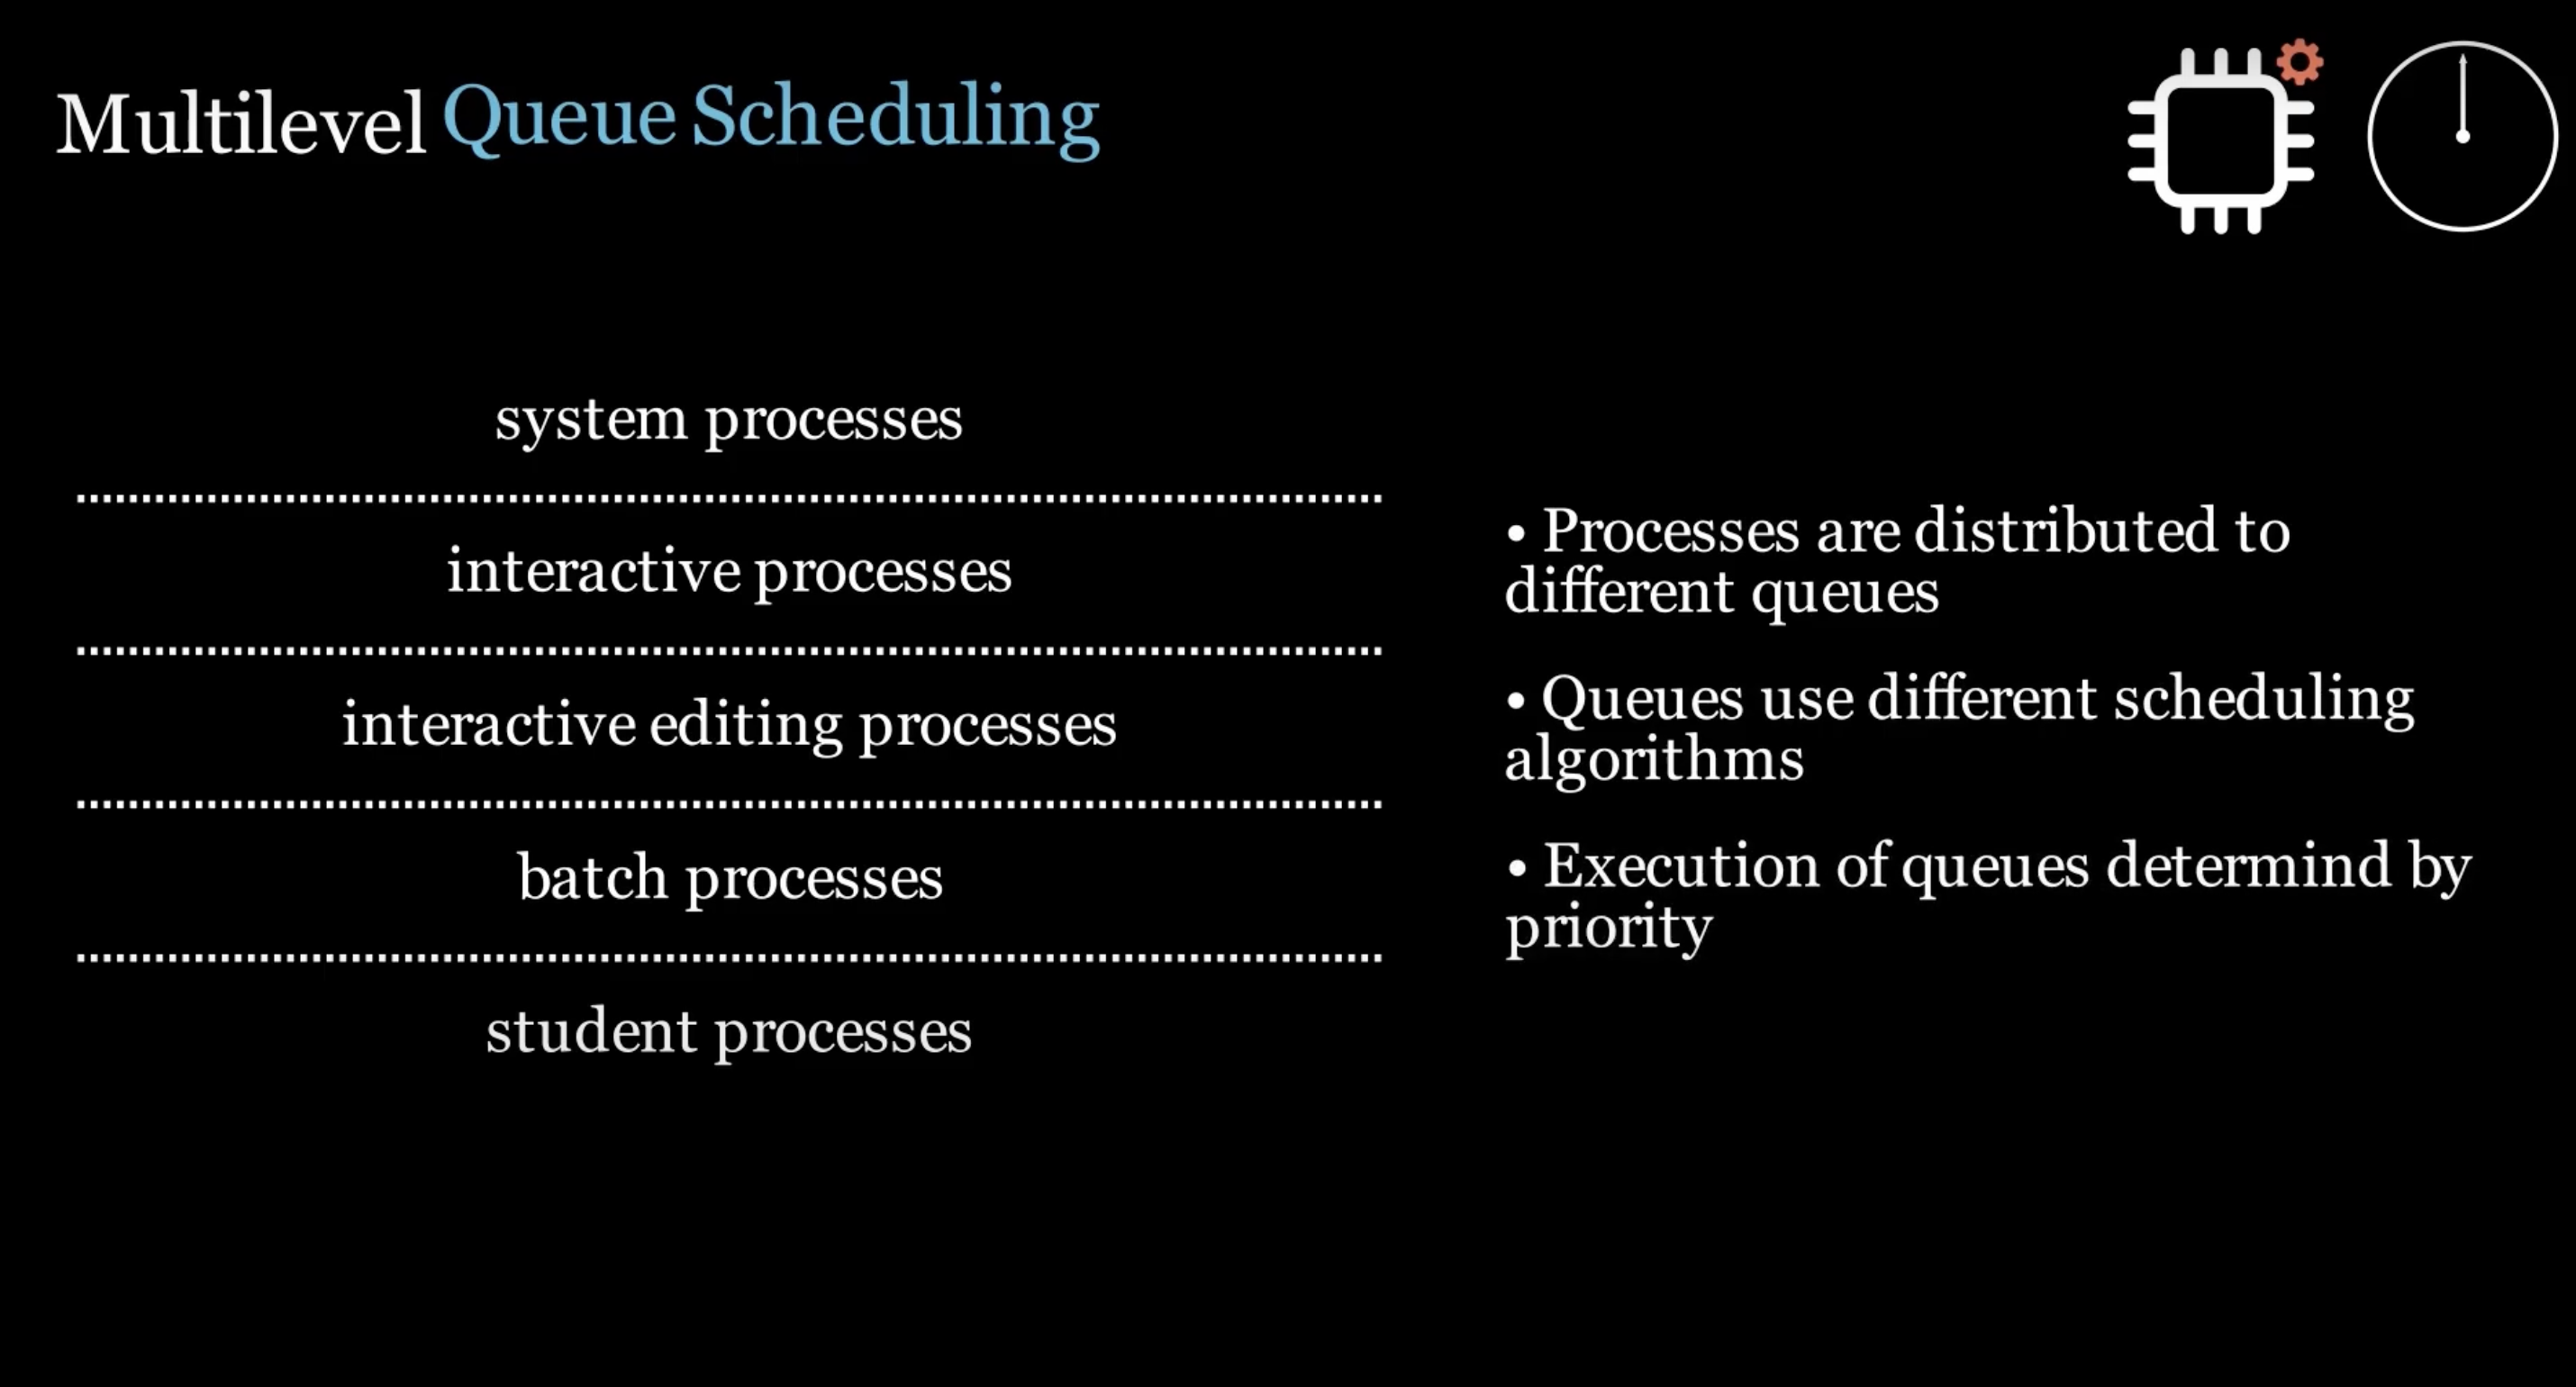
\includegraphics[width=0.8\linewidth]{img/screen_text.png} 
	\caption{Die Szene zur Erklärung des \ac{MLQ}-Algorithmus zeigt die Kombination zwischen animierten Bildinformationen mit unterstützendem Text.}
	\label{fig:screen_text} 
\end{figure}

% Komposition von Objekten
Des Weiteren bietet die Gestaltpsychologie von Kurt Koffka wertvolle Einsichten zur visuellen Wahrnehmung, insbesondere wie Menschen visuelle Informationen verarbeiten und interpretieren \autocite{koffka_principles_1999}. So spielt die Hierarchie visueller Elemente eine entscheidende Rolle, indem diese das Hervorheben wichtiger Inhalte ermöglicht und die Aufmerksamkeit des Lernenden gezielt lenken kann. Die Führung des Blicks durch eine durchdachte Komposition und die strategische Verwendung von Leerflächen können ebenfalls dazu beitragen, die kognitive Belastung zu minimieren und die Aufnahme der Lerninhalte zu erleichtern \autocite{koffka_principles_1999}.
Indem diese beispielhaft genannten Prinzipien berücksichtigt werden, können Lehrvideos nicht nur ästhetsich ansprechend sein, sondern auch die Lernprozesse durch eine verbesserte visuelle Wahrnehmung unterstützen. Beispielsweise werden die Funktionsweisen der unterschiedlichen Scheduling Algorithmen innerhalb unseres Lehrvideos durch sich bewegende Prozesse dargestellt, welche durch eine sich drehende \ac{CPU} abgearbeitet werden. Dies unterstützt dem Zuschauer Zusammenhänge leichter und schneller zu verstehen. 

Auch die Gestaltprinzipien der Wahrnehmung von Max Wertheimer, welche von der Gestaltpsychologie abzugrenzen sind, bieten Einsichten für die Gestaltung von Bildungsanimationen \autocite{wertheimer_untersuchungen_2017}. Diese Prinzipien, wie die Gruppierung von Elementen nach Nähe oder Ähnlichkeit, können genutzt werden, um Beziehungen und Strukturen zu verdeutlichen. So kann beispielsweise das Prinzip der Nähe dazu verwendet werden, um zu zeigen, wie verschiedene Elemente miteinander in Beziehung stehen. 

% Screenshot einfügen mit Beschreibung. Etwas mit Grafik & animiertem Text dazu
\begin{figure}[h]
	\centering
	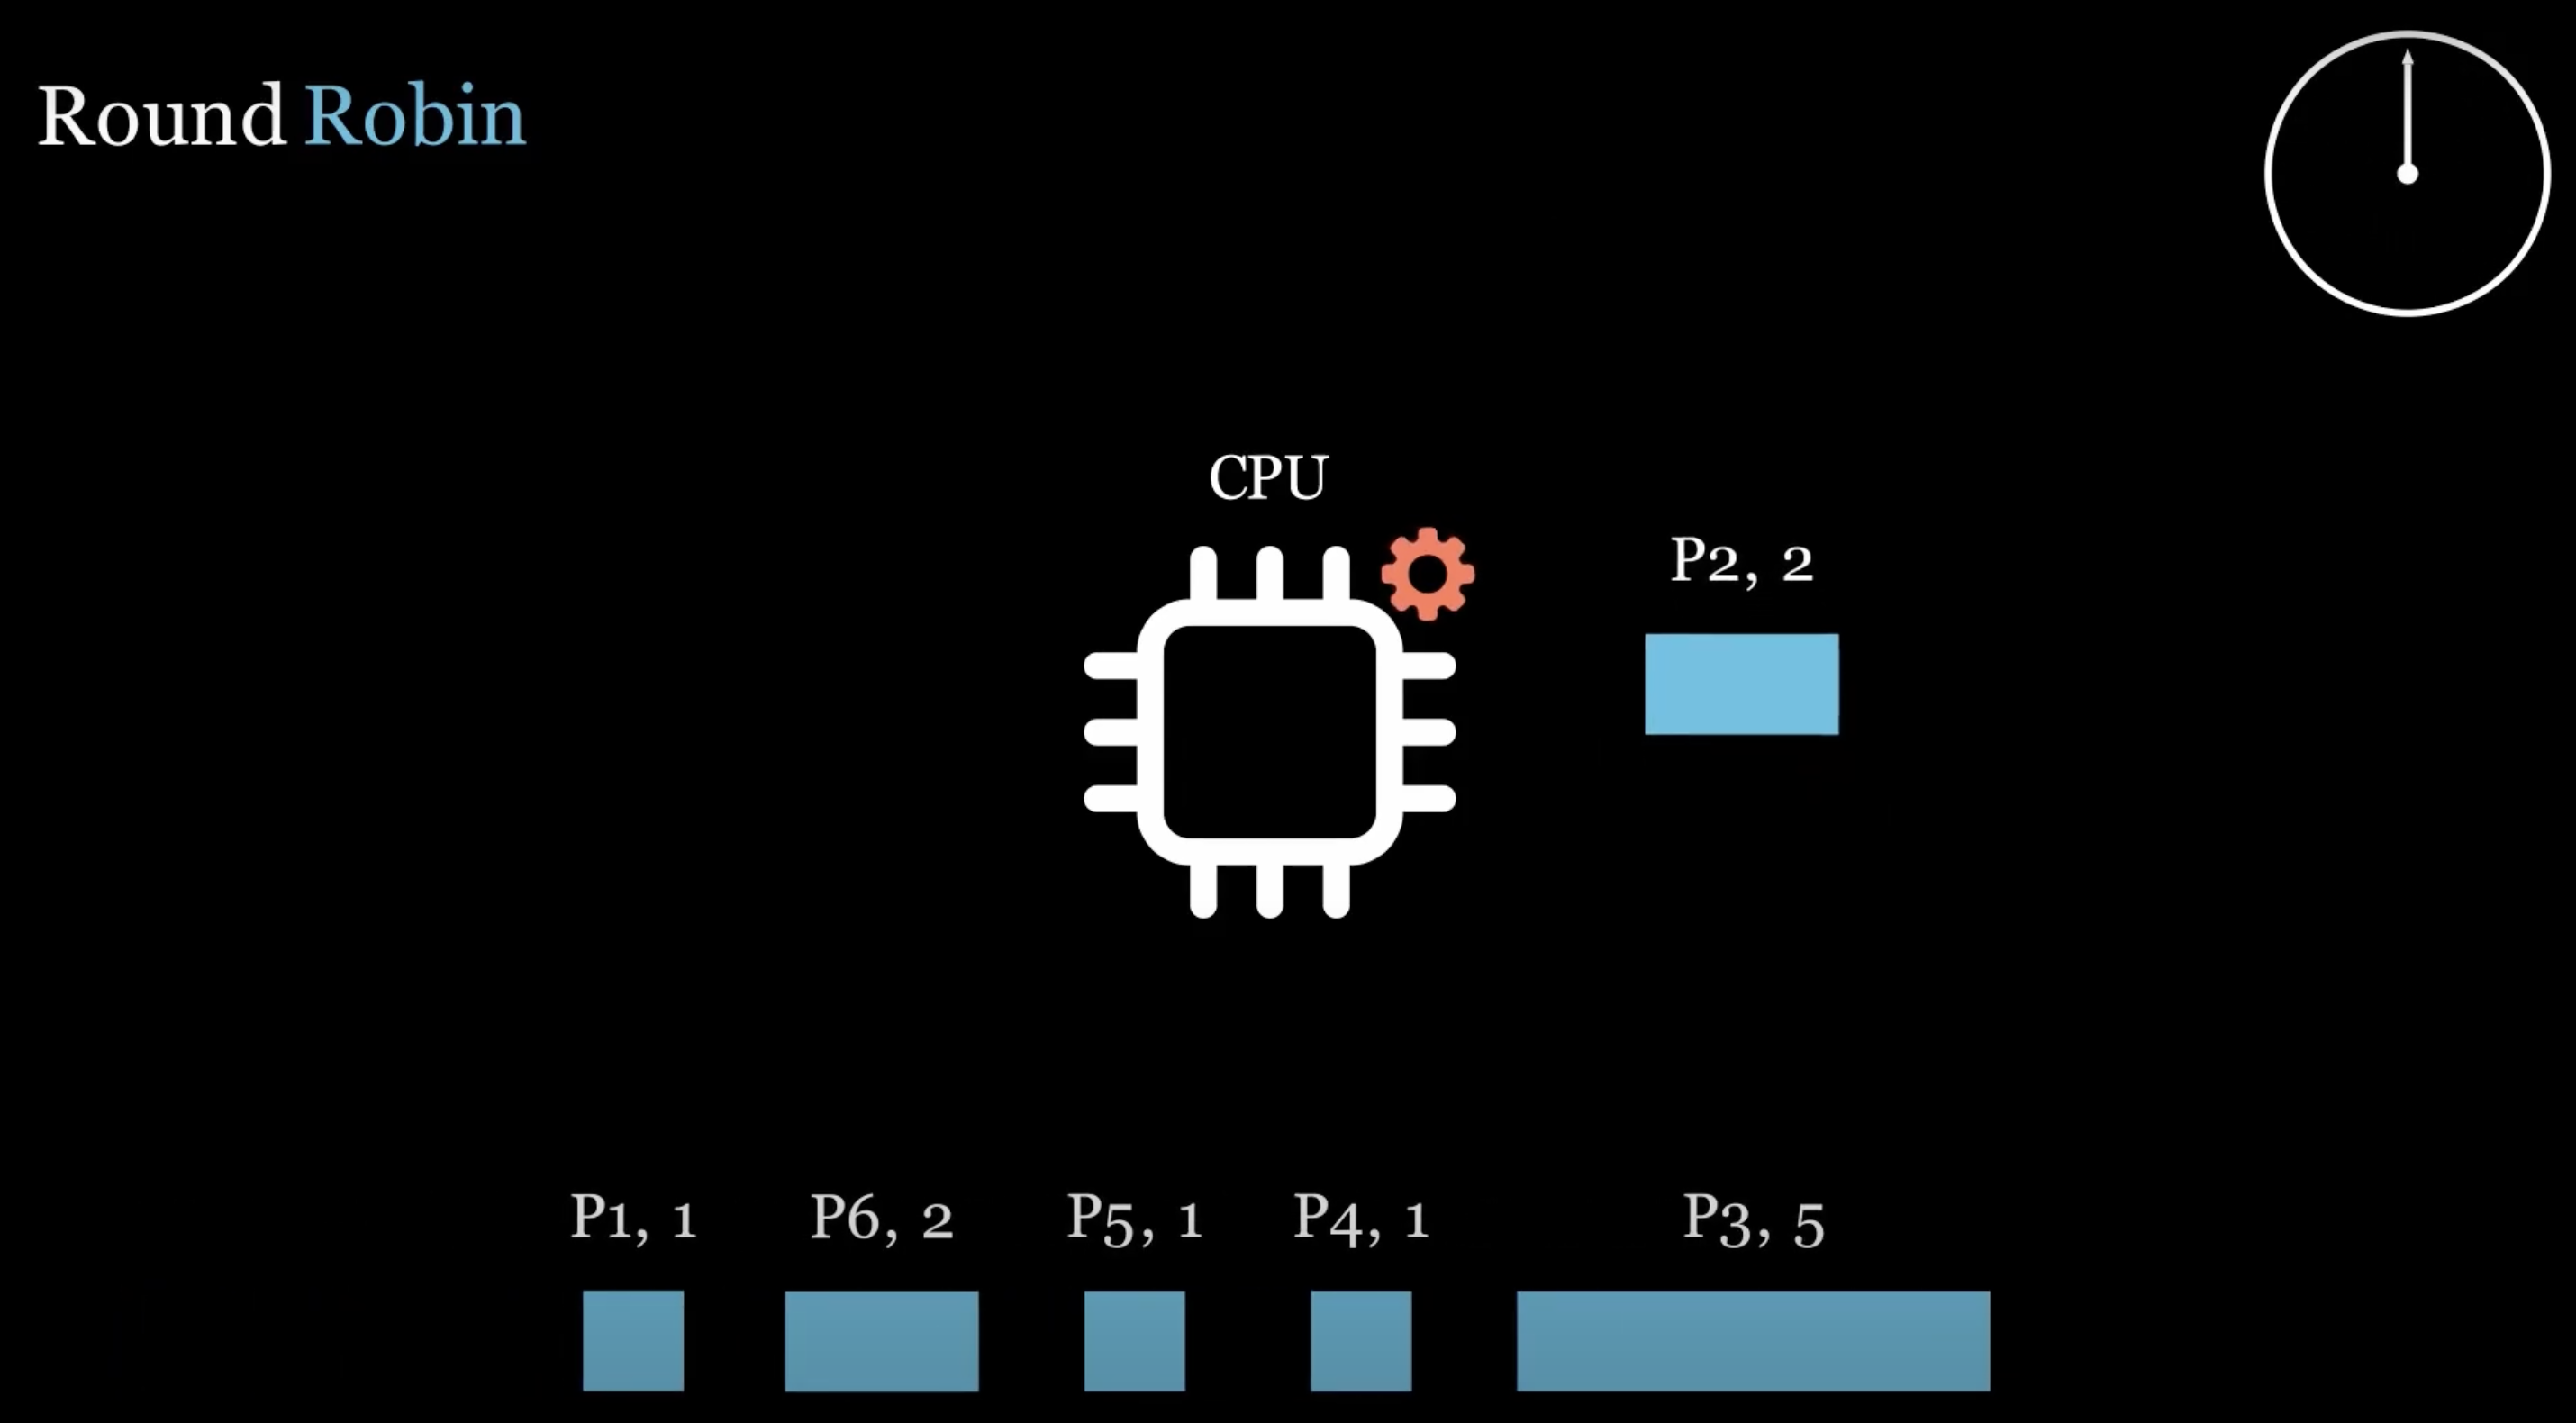
\includegraphics[width=0.8\linewidth]{img/screen_komposition.png} 
	\caption{Wird ein Prozess von der \ac{CPU} abgearbeitet, reduziert sich die Breite des Prozesses, um eine Verringerung der verbleibenden Bearbeitungszeit darzustellen.}
	\label{fig:screen_komposition} 
\end{figure}


%\textbf{Farbgestaltung}:
Neben der Wichtigkeit von Animationen und Komposition ist eine geschickte Auswahl der gewählten Farben ebenso essentiell. Laut der Farbtheorie kann die Auswahl von Farben und Kontrasten dabei unterstützen, wichtige Informationen hervorzuheben und die visuelle Erfahrung, und somit die vermittelten Inhalte, der Lernenden zu bereichern \autocite{ballard_art_1964}. Das von uns erstellte Lehrvideo versucht eine konsistente farbliche Harmonie zu bewirken, was durch die kontinuierliche Verwendung einer abgestimmten Farbpalette erreicht wird. Teilweise werden zudem wichtige Komponenten mithilfe von Sekundärfarben hervorgehoben, wie beispielsweise in Abbildung \ref{fig:screen_farben} das Erscheinen eines neuen Prozesses durch die Farbe orange betont wird. 

% Screenshot einfügen von "Animation". Wie ein Algorithmus etwas verarbeitet oder so
\begin{figure}[h]
	\centering
	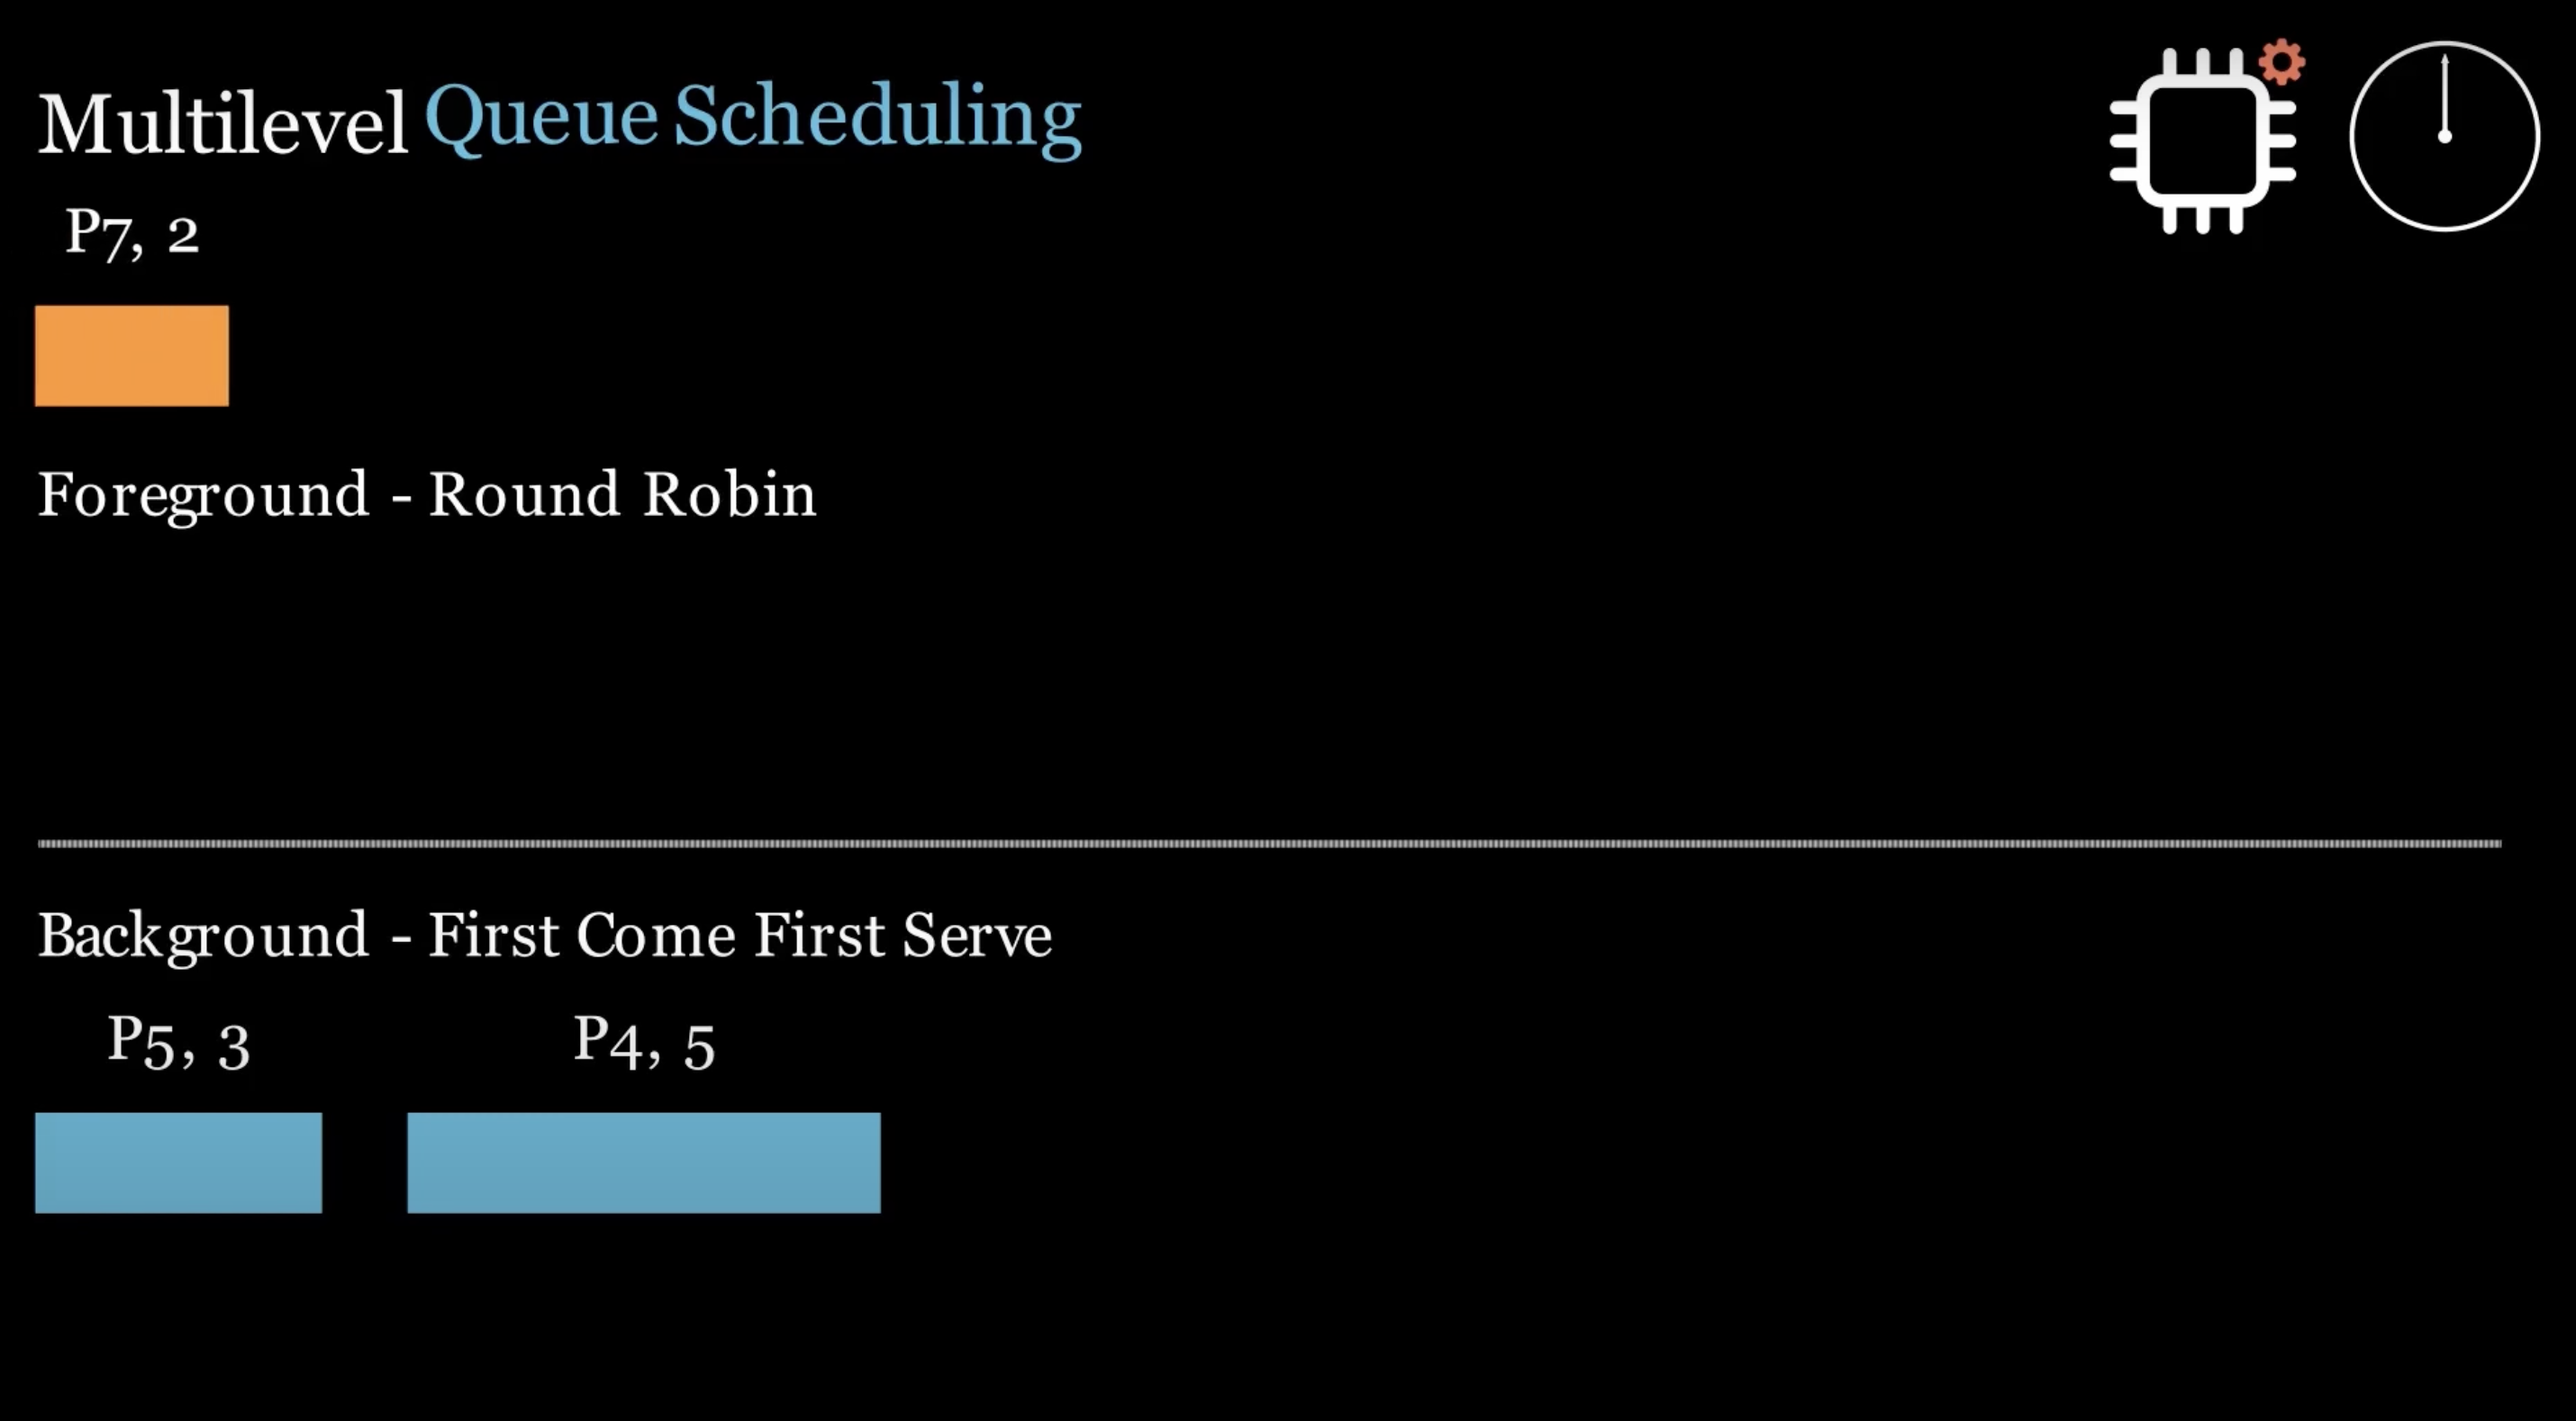
\includegraphics[width=0.8\linewidth]{img/screen_farben.png} 
	\caption{In der \ac{MLQ} Szene wird ein neu hinzukommender Prozess mithilfe einer orangenen Farbe für den Lernenden hervorgehoben.}
	\label{fig:screen_farben} 
\end{figure}


%\textbf{Auditive Unterstützung}:
Abgesehen der zuvor beschriebenen visuellen Komponenten nimmt die Musik ebenfalls eine zentrale Rolle ein, da diese entscheidend zur Steigerung der Aufmerksamkeit, zur Steuerung der Stimmung und zur Verbesserung des Verständnis beitragen kann. John A. Sloboda betont in "The Musical Mind: The Cognitive Psychology of Music", dass Musik und Soundeffekte nicht nur die emotionale Reaktion der Zuschauer beeinflussen, sondern auch deren Engagement und Erinnerungsvermögen fördern können \autocite{sloboda_musical_1986}. Durch den gezielten Einsatz von Musik können bestimmte Stimmungen erzeugt oder verstärkt werden, was die Aufnahme und Verarbeitung von Informationen unterstützt. Ebenso können Soundeffekte dazu dienen, wichtige Momente hervorzuheben und den Lernenden dazu anzuregen, ihre volle Aufmerksamkeit auf spezifische Aspekte des Videos zu richten \autocite{sloboda_musical_1986}. 
So versucht unser Lehrvideo mit einer ansprechenden und beruhigenden audiovisellen Erlebnis die kognitive Verarbeitungsfähigkeit der Lernenden zu fördern und ein effektiveres Lernerlebnis zu bieten. 


%\textbf{Storyline und Stringenz}:
Nachdem nun visuelle und auditive Aspekte beschrieben wurden, ist die Erwähnung anderer Aspekte wie der Integration von Storytelling innerhalb des Lehrvideos essentiell. Auch wenn es sich hierbei nicht um eine Art der Visualisierung handelt, kann hierduch eine eine emotionale Verbindung zum Lehrmaterial hergestellt werden, worduch dieses zugänglicher und einprägsamer wird. Roger C. Schank unterstreicht in "Tell me a story: A new look at real and artificial memory" die Relevanz von Geschichten auf das menschliche Verständnis und Erinnerungsvermögen \autocite{schank_tell_1990}. Indem Lehrvideos eine solche narrative Stringenz aufweisen, bei welcher beispielsweise die Optimierung einer ToDo-Liste durch den Einsatz eines Betriebssystem-Scheduling-Algorithmus als durchgängige Story dient, kann das Interesse und die Motivation der Zuschauer gesteigert werden. Die in unserem Lehrvideo dargestellte ToDo-Liste enthält hierbei bewusst Einträge, welche eine persönliche Relevanz für den Zuschauer haben, um eine emotionale Verbindung herzustellen. Durch diesen Ansatz wird zu Beginn und am Ende des Videos nicht nur die Aufmerksamkeit gefesselt, sondern es wird auch ein Rahmen geschaffen, der das Verständnis und die Merkfähigkeit der vermittelten Inhalte maßgeblich verbessert.


\begin{figure}[h]
	\centering
	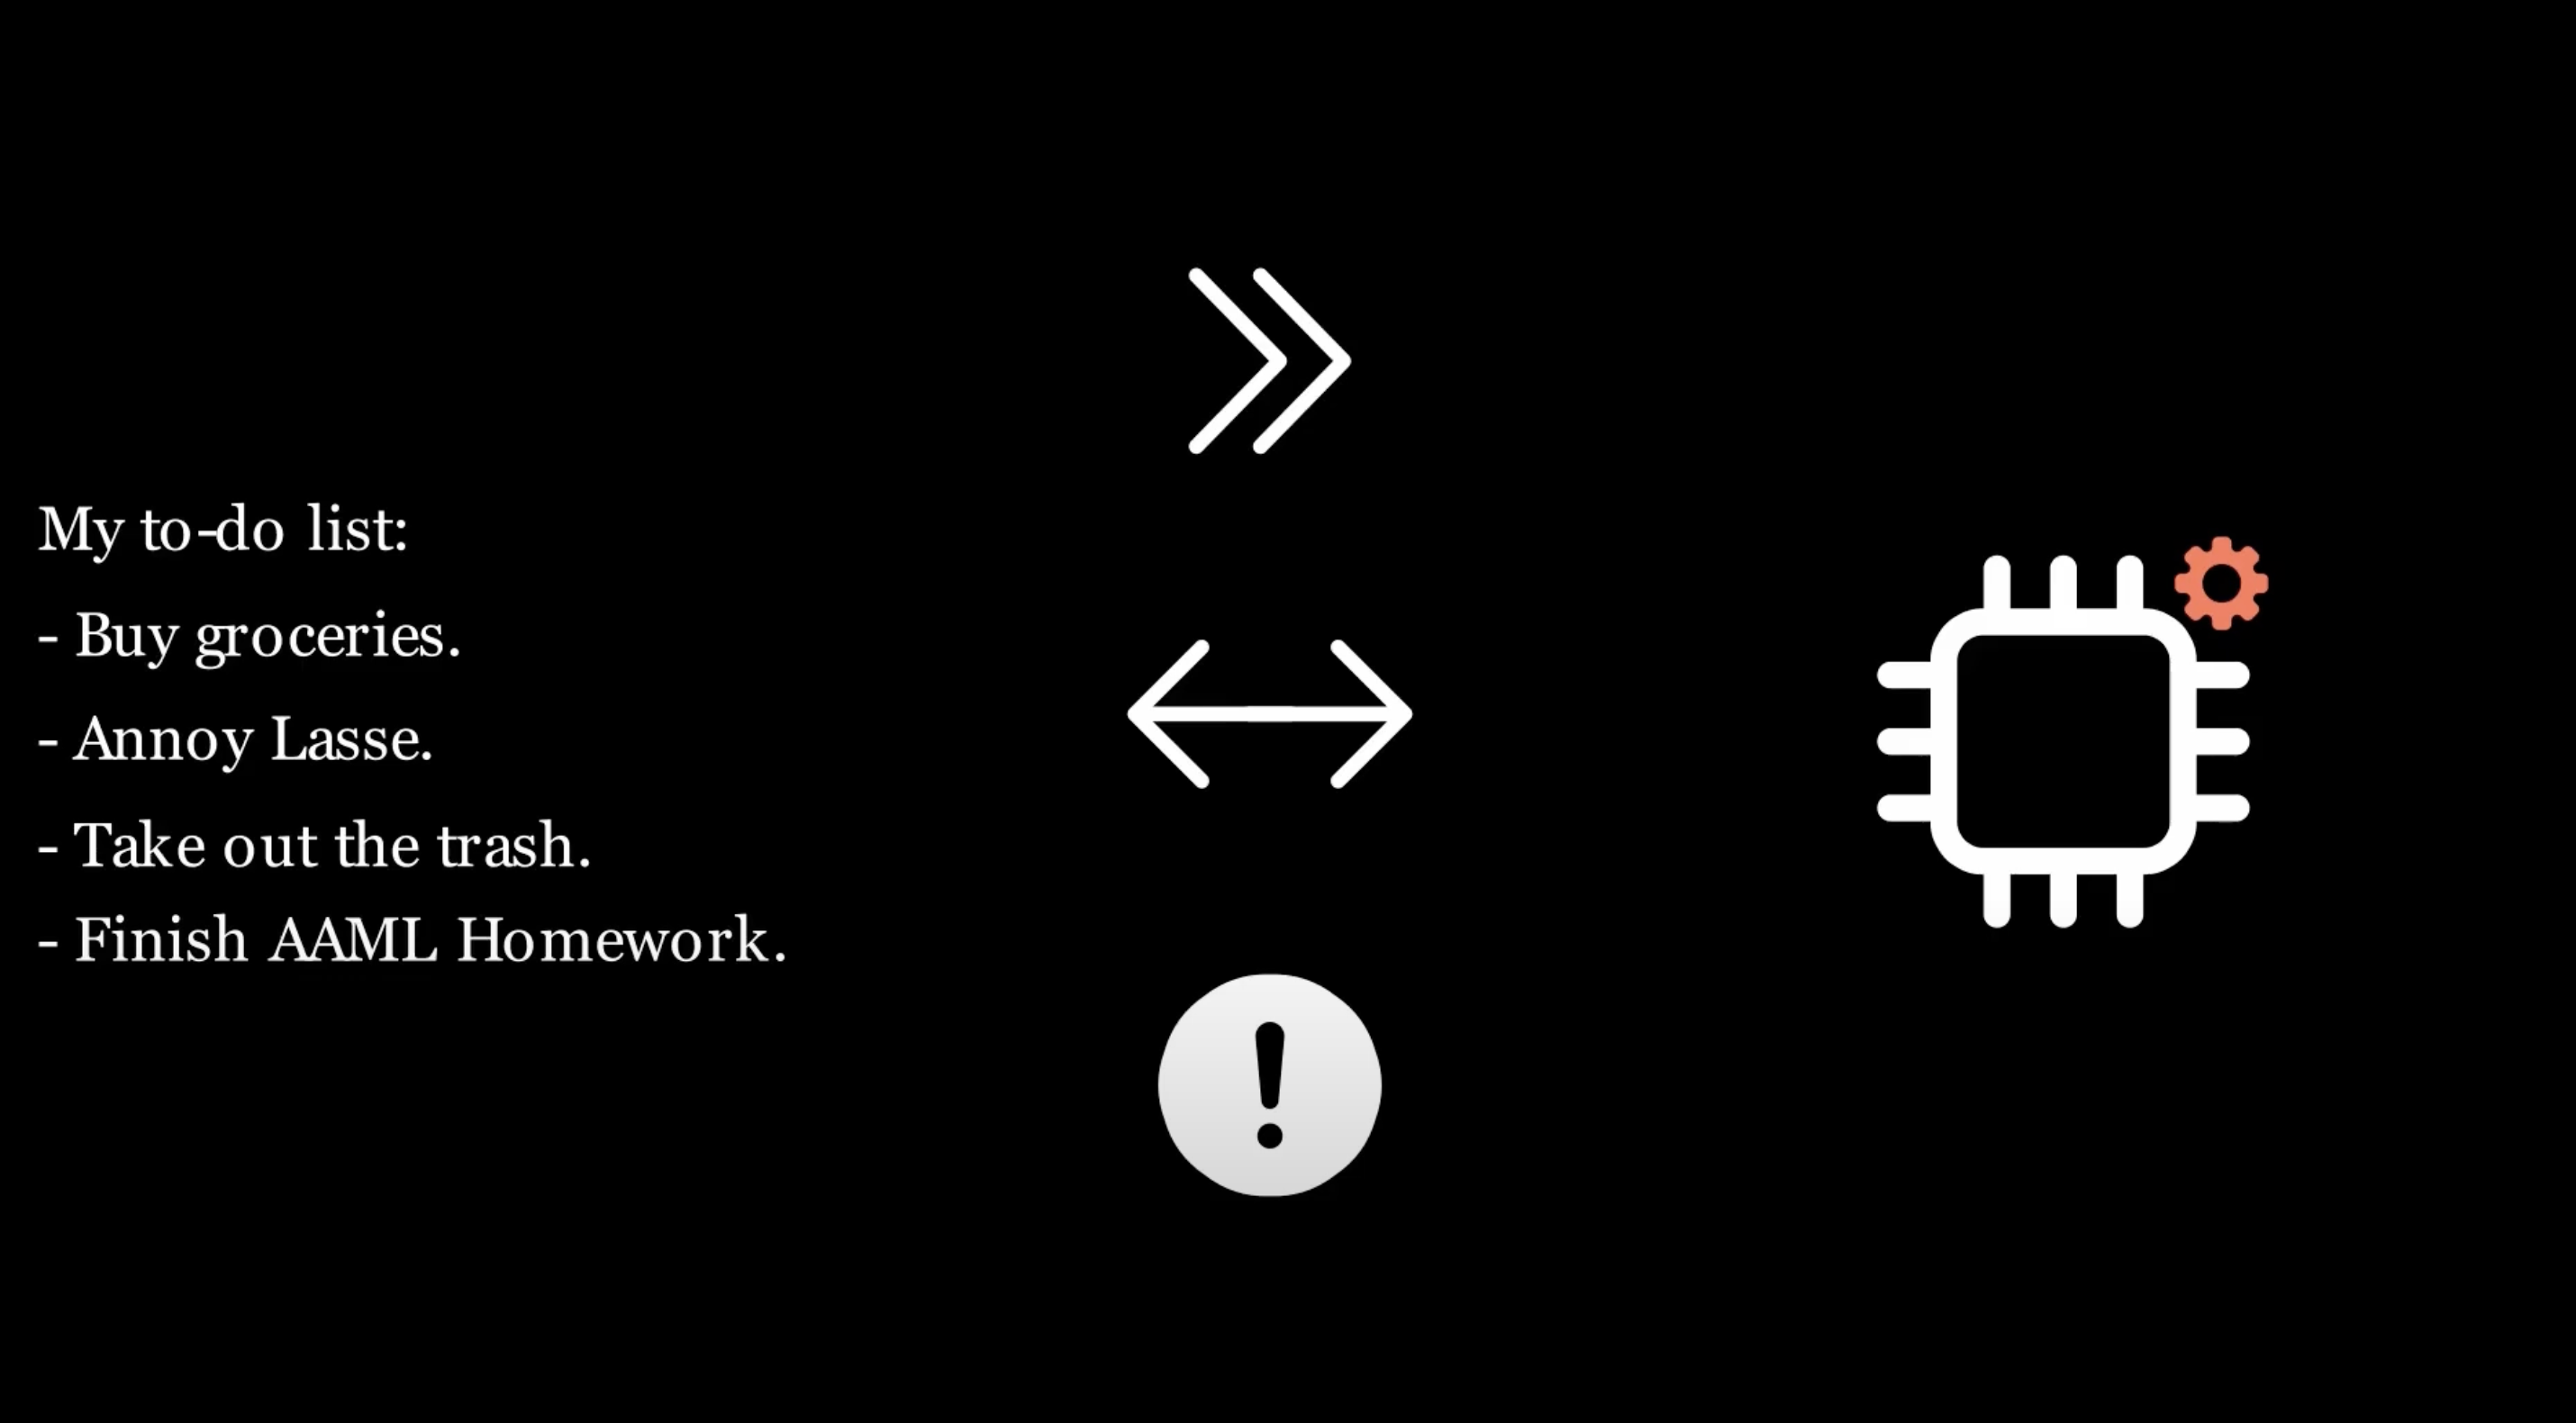
\includegraphics[width=0.8\linewidth]{img/screen_todo.png} 
	\caption{Die ToDo Liste dient als Einleitung und Abschluss des Lehrvideos, um eine inhaltliche Stringenz zu bewirken.}
	\label{fig:screen_todo} 
\end{figure}


Nachdem nun auf die theoretischen Grundlagen der Visualisierung eingegangen wurde, beschäftigen sich die folgenden Kapitel mit der Erklärung verwendeter Scheduling Algorithmen und einer anschließenden Performance Analyse dieser im Vergleich.

